% Autor: Romain Schmitz
% Zuletzt ge�ndert: 17.1.2007

\documentclass{beamer}
\usepackage[latin1]{inputenc}

\usepackage{beamerthemesplit}

\usepackage{graphicx}
\usepackage{multicol}
\usepackage{listings}
\usepackage{fancybox}


\author{Romain Schmitz}

\title{Architektur der PC-Uhr}

\date{\today}

\begin{document}
\lstset{
		numbers=left,
		numbersep=10pt,
		numberstyle=\tiny,
		frame=single,
		basicstyle=\tt\scriptsize,
		keywordstyle=\bz,
		stringstyle=\it
		commentstyle=\sl
		captionpos=b}

\frame{\titlepage}

\section{�bersicht}
\frame
{
\tableofcontents
}

\section{Architektur}

\frame
{
\textbf{Software-Architektur}

\begin{itemize}
\item<2->[]
	%\begin{quote}
	\shadowbox{\parbox{9cm}{Strukturierte oder hierarchische Anordnung der
	System\-komponenten sowie die Beschreibung ihrer Beziehungen.

	\scriptsize{(Def. nach Helmut Balzert)}}}
	%\end{quote}
\end{itemize}
}

\subsection[Erstes Design (syntaktisch fehlerhaft)]{Erstes Design}
\frame
{
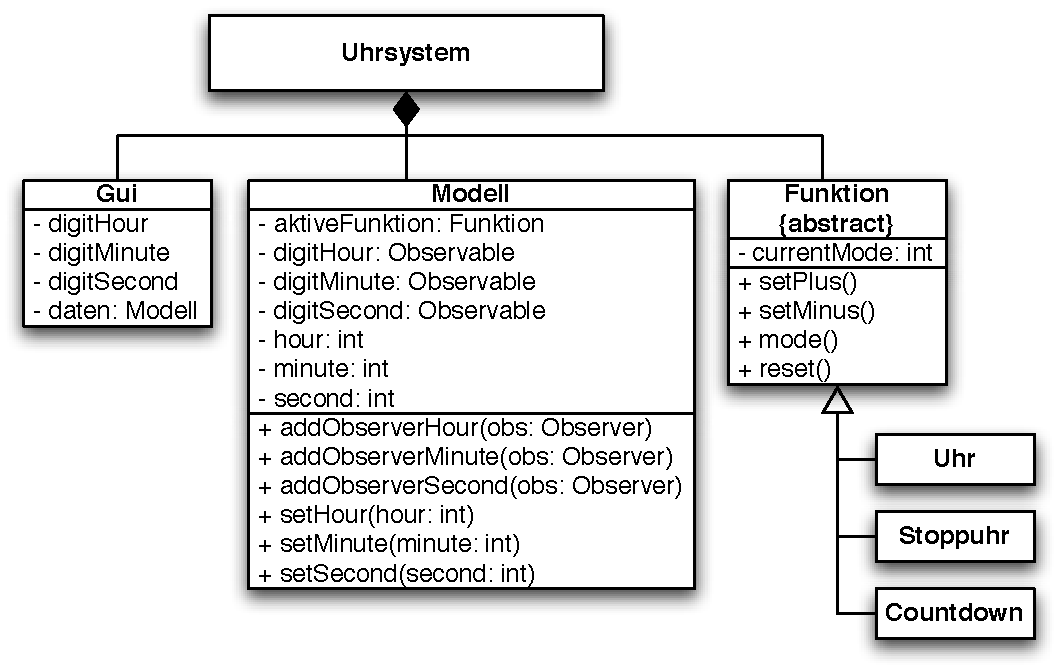
\includegraphics[scale=0.5]{pix/Design1}
}

\subsection[1. Iteration (syntaktisch fehlerhaft)]{1. Iteration}
\frame
{
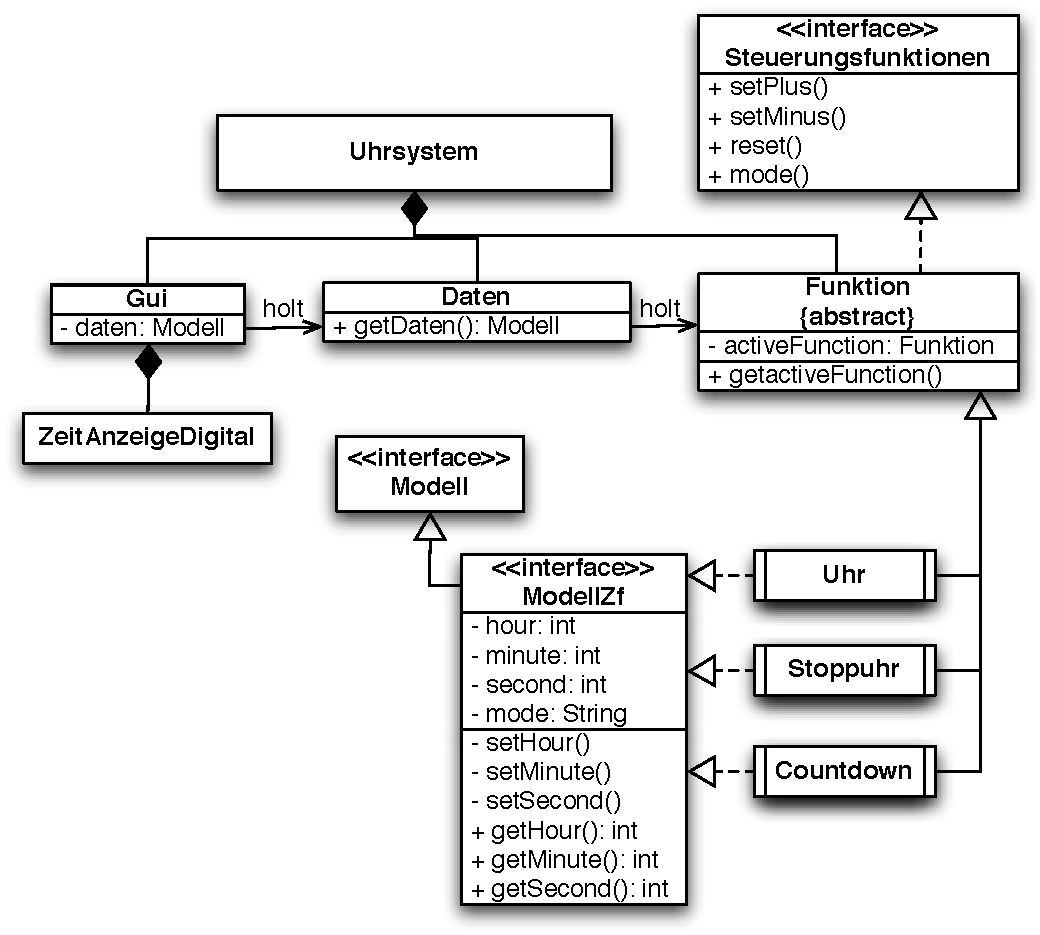
\includegraphics[scale=0.5]{pix/Design2}
}

\subsection[2. Iteration (syntaktisch fehlerhaft)]{2. Iteration}
\frame
{
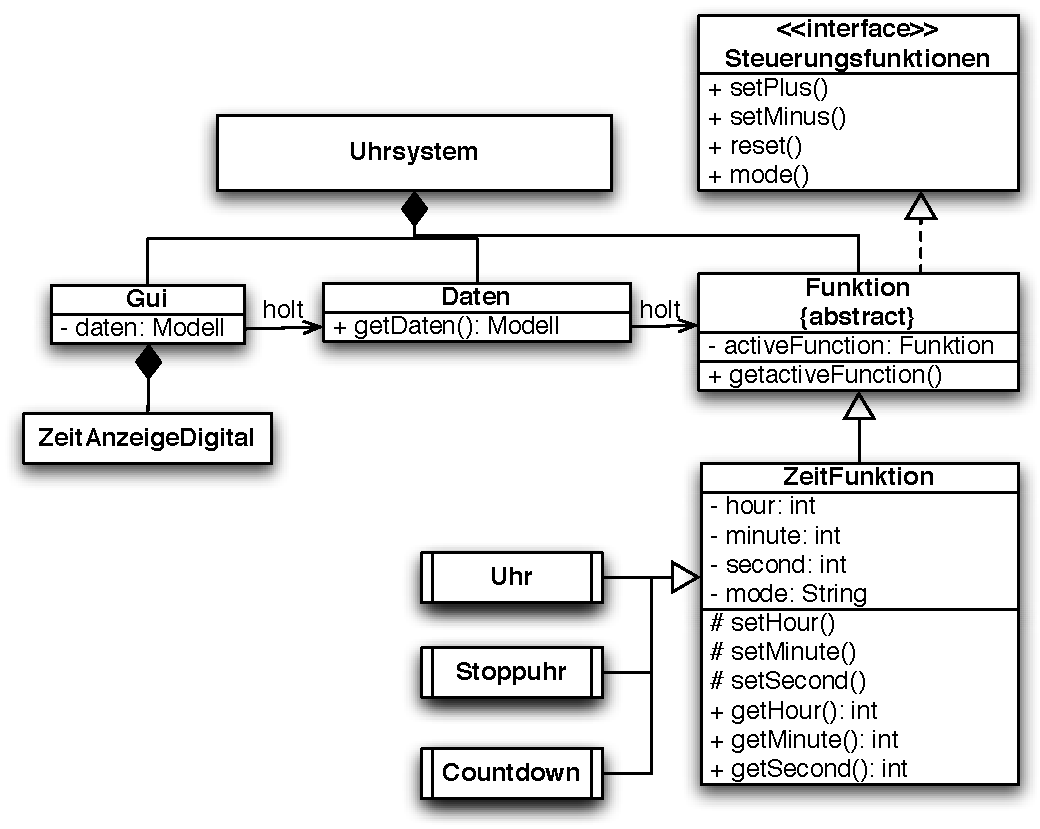
\includegraphics[scale=0.5]{pix/Design3}
}

\subsection{3. Iteration}
\frame
{
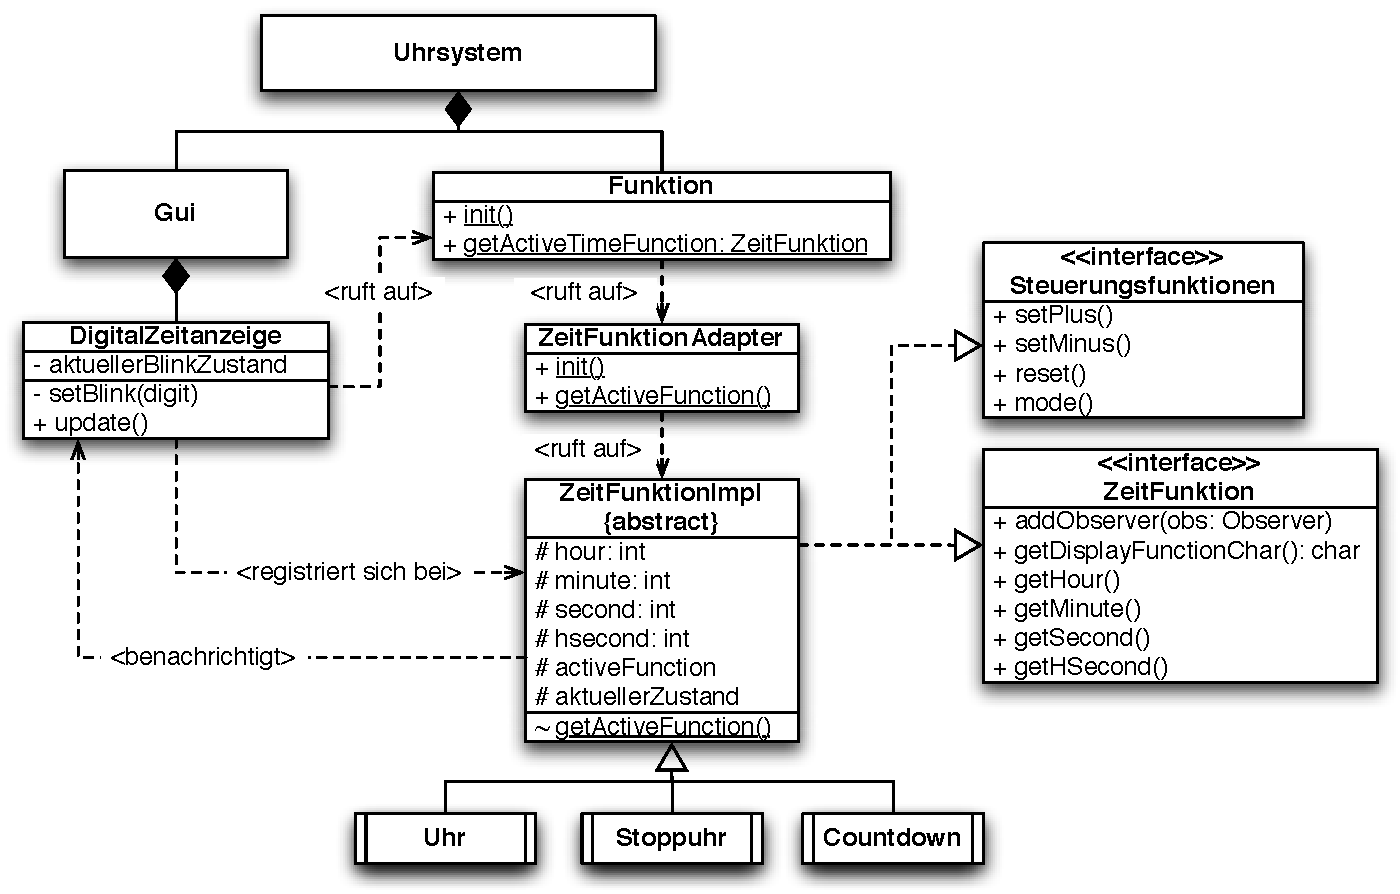
\includegraphics[scale=0.5]{pix/Design4}
}

\section{Design-Pattern 1}

\frame
{
\textbf{Design-Pattern}

\begin{enumerate}
\item<2-> beschreiben L�sungen f�r Entwurfsprobleme.
\item<3-> vereinfachen Diskussionen zwischen Entwicklern.
\end{enumerate}
}

\subsection*{Interface-Pattern}
\frame
{
%\frametitle{Interface-Pattern}
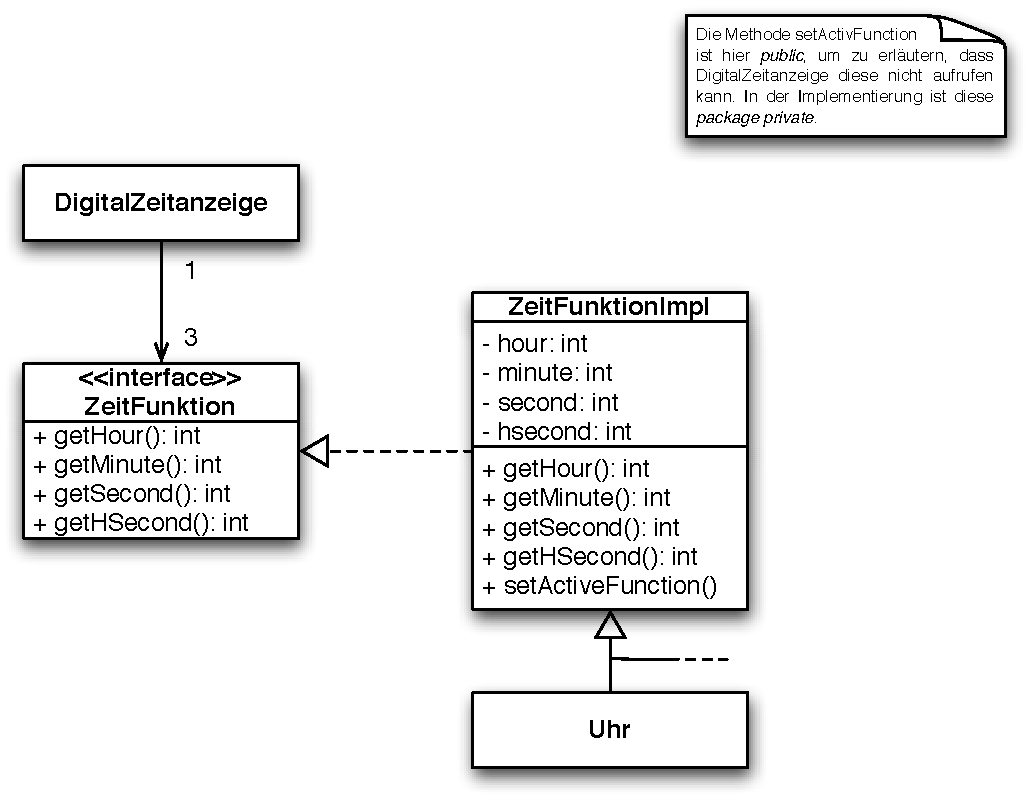
\includegraphics[scale=0.5]{pix/Interface-Pattern}
}


\subsection*{Observer-Pattern}
\frame
{
%\frametitle{Observer-Pattern}
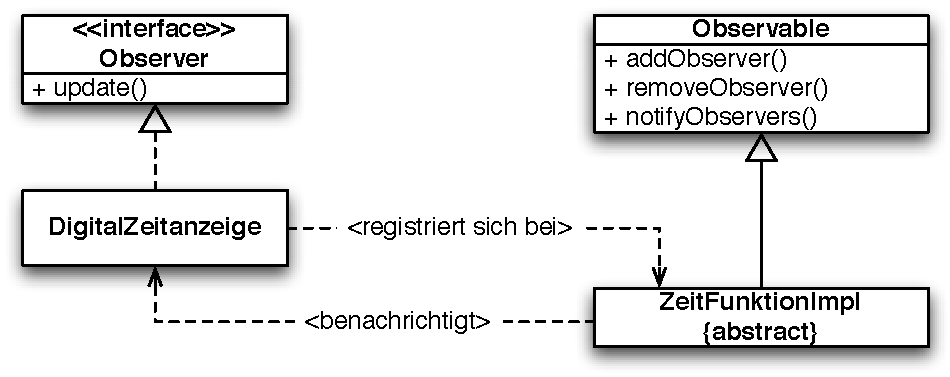
\includegraphics[scale=0.6]{pix/Observer-Pattern}
}

\subsection*{Immutable-Pattern}
\begin{frame}[fragile]
%\frametitle{Immutable-Pattern}

%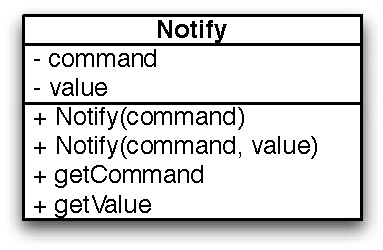
\includegraphics[scale=0.6]{pix/Immutable}

\setlength{\columnseprule}{0pt}
\setlength{\columnsep}{0pt}
\begin{multicols}{2}
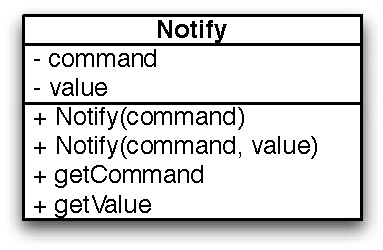
\includegraphics[scale=0.6]{pix/Immutable}
\vspace{5cm}
\begin{scriptsize}
\begin{verbatim}
public class Notify {	

    private commands command = null;
    private Object value = null;	
			
    public Notify(commands command) 
    {
        this.command = command;
    }	
    
    public Notify( commands command, 
                   Object value) 
    {
        this.command = command;
        this.value = value;
    }
    
    ...
}
\end{verbatim}
\end{scriptsize}
\end{multicols}

%\begin{lstlisting}[language=Java,caption=test]
%public class Notify {	
%	private commands command = null;
%	private Object value = null;	
%	
%	public Notify(commands command) {
%		this.command = command;
%	}	
%	
%	public Notify(commands command, Object value) {
%		this.command = command;
%		this.value = value;
%	}	
%	
%	public commands getCommand() {
%		return this.command;
%	}		
%	
%	public Object getValue() {
%		return this.value;
%	}		
%}
%
%\end{lstlisting}

\end{frame}


%\subsection*{Factory-Pattern}
%\frame
%{
%%\frametitle{Factory-Pattern}
%}



%\subsection*{State-Pattern}
%\frame
%{
%%\frametitle{State-Pattern}
%}


%
%\subsection*{Adapter-Pattern}
%\frame
%{
%%\frametitle{Adapter-Pattern}
%}

\section{Design-Pattern 2}
\frame
{
Details zum State-Pattern
\begin{itemize}
\item<2-> f�r das Blinken der Digits der Digitalanzeige,
\item<3-> f�r die Uhrfunktionen.
\end{itemize}
}


\subsection*{State-Pattern f�r das Blinken}
\frame
{
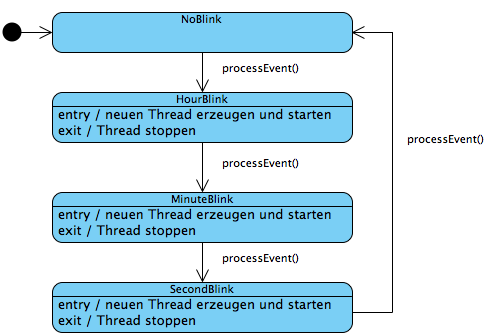
\includegraphics[scale=0.5]{pix/BlinkZustandsdiagramm}
}

\frame
{
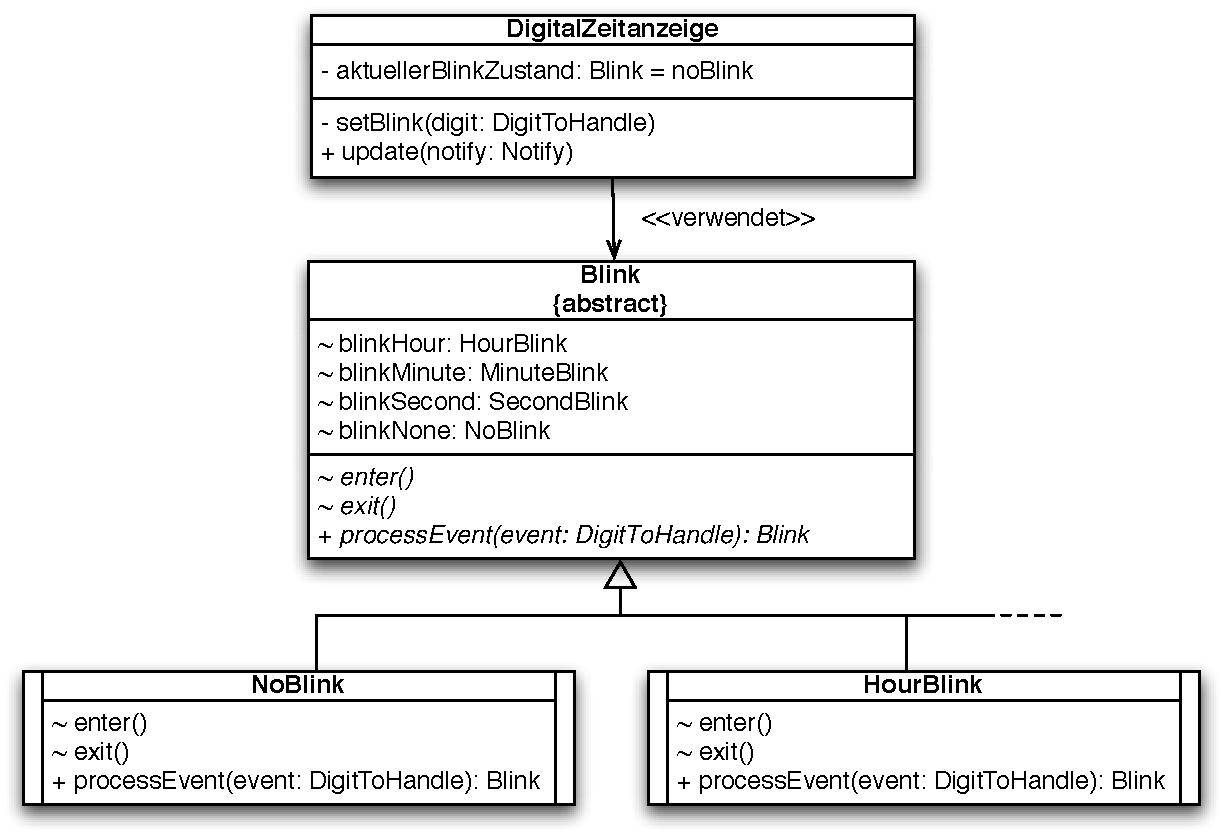
\includegraphics[scale=0.5]{pix/State-Pattern}
}

\subsection*{Verschachteltes State-Pattern f�r die Uhrfunktionen}
\frame
{
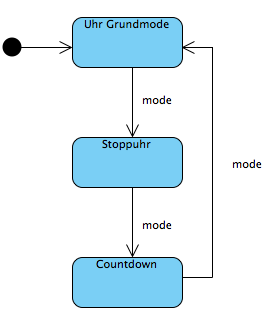
\includegraphics[scale=0.5]{pix/Uhrzustandsdiagramm1}
}

\frame
{
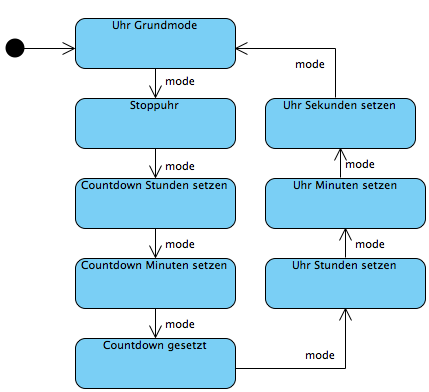
\includegraphics[scale=0.5]{pix/Uhrzustandsdiagramm2}
}

\frame
{
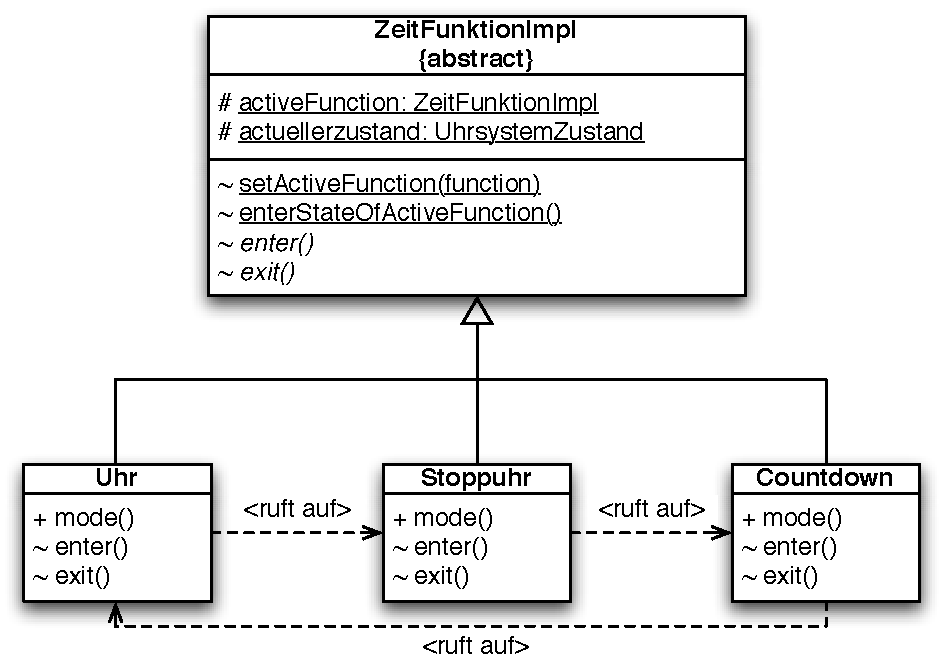
\includegraphics[scale=0.6]{pix/State-Pattern2}
}

\section{Design-Pattern 3}
\subsection*{Weitere Design-Pattern}
\frame
{
Weitere Design-Pattern sind:
\begin{itemize}
    \item<2-> Factory
    \item<3-> Delegate
    \item<4-> Visitor
    \item<5-> Composite
    \item<6-> Chain of Responsibility
    \item<7-> Little Language
    \item<8-> ...
\end{itemize}
}

\end{document}
